\documentclass[border=2pt]{standalone}
\usepackage[T1]{fontenc}
\usepackage{lmodern,amsmath,amssymb,tikz}
\begin{document}
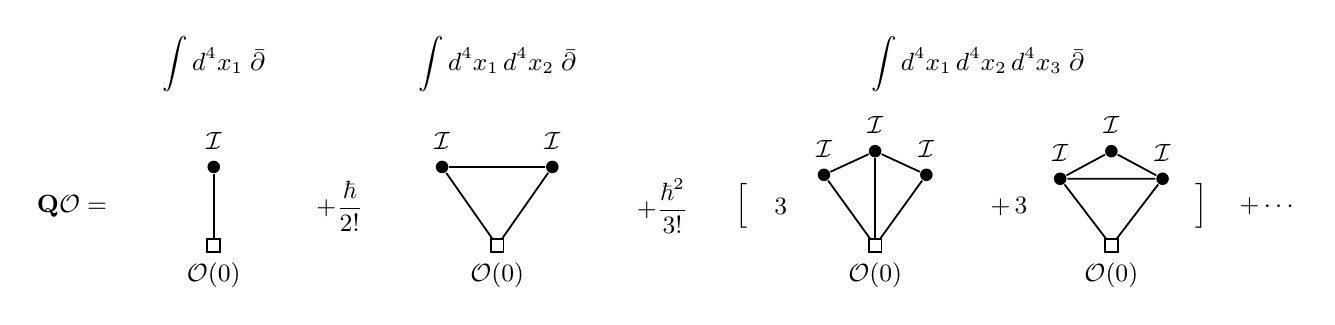
\begin{tikzpicture}[x=1cm,y=1cm,font=\small,
 dot/.style={circle,fill=black,inner sep=1.6pt},
 root/.style={rectangle,draw,fill=white,inner sep=2.3pt},
 every path/.style={line width=.65pt}]
\node at (-1,.5) {$\mathbf Q\mathcal O=$};
\node at (.8,2.3) {$\displaystyle\int d^4x_1\;\bar\partial$};
\node[dot,label=above:{$\mathcal I$}] (a) at (.8,1) {};
\node[root,label=below:{$\mathcal O(0)$}] (o) at (.8,0) {};
\draw (a)--(o);
\node at (2.4,.5) {$+\dfrac{\hbar}{2!}$};
\node at (4.4,2.3) {$\displaystyle\int d^4x_1\,d^4x_2\;\bar\partial$};
\node[dot,label=above:{$\mathcal I$}] (a) at (3.7,1) {};
\node[dot,label=above:{$\mathcal I$}] (b) at (5.1,1) {};
\node[root,label=below:{$\mathcal O(0)$}] (o) at (4.4,0) {};
\draw (a)--(b)--(o)--(a);
\node at (6.5,.5) {$+\dfrac{\hbar^2}{3!}$};
\node at (10.5,2.3) {$\displaystyle\int d^4x_1\,d^4x_2\,d^4x_3\;\bar\partial$};
\node at (7.5,.5) {$\Bigl[$};
\node at (8,.5) {$3$};
\begin{scope}[xshift=9.2cm]
 \node[dot,label=above:{$\mathcal I$}] (a) at (-.65,.9) {};
 \node[dot,label=above:{$\mathcal I$}] (b) at (0,1.2) {};
 \node[dot,label=above:{$\mathcal I$}] (c) at (.65,.9) {};
 \node[root,label=below:{$\mathcal O(0)$}] (o) at (0,0) {};
 \draw (a)--(b)--(c)--(o)--(a); \draw (b)--(o);
\end{scope}
\node at (10.9,.5) {$+\,3$};
\begin{scope}[xshift=12.2cm]
 \node[dot,label=above:{$\mathcal I$}] (a) at (-.65,.85) {};
 \node[dot,label=above:{$\mathcal I$}] (b) at (0,1.2) {};
 \node[dot,label=above:{$\mathcal I$}] (c) at (.65,.85) {};
 \node[root,label=below:{$\mathcal O(0)$}] (o) at (0,0) {};
 \draw (a)--(b)--(c)--(o)--(a)--(c);
\end{scope}
\node at (13.35,.5) {$\Bigr]$};
\node at (14.2,.5) {$+\cdots$};
\end{tikzpicture}
\end{document}
